\section{První verze}

První čistě mechanická varianta vznikla začátkem srpna 2019, brzy po výše popsané elektronické variantě.
Měla stále poměrně klasický vzhled trezoru -- zamykatelná skříňka, která obsahovala dvě kódovací kola, která ovládala možnost pohybu jednoduché západky. %todo lepší formulaci
Na rozdíl od její elektronické před\-chůd\-ky\-ně bylo vše zajímavé uvnitř dveří. Také byla určená jako základ pro případný upgrade na elektronickou
variantu. Na podobné vylepšení mělo stačit odstranění kódovacích kol a přidělání elektronické části. Toto sice fungovalo obstojně, zároveň 
i jako motivace, ale kvůli pozdější změně konceptu mechanizmu tento nápad padl.
Tato varianta se také ukázala jako nevhodná (kvůli přílišným nárokům na přesnost) pro stavbu s malými dětmi, pro které byla určena jakožto předstupeň 
k variantě elektronické (která vyžaduje i znalosti nebo alespoň ochotu k učení se programování).

\begin{figure}[htbp]
    \centering
    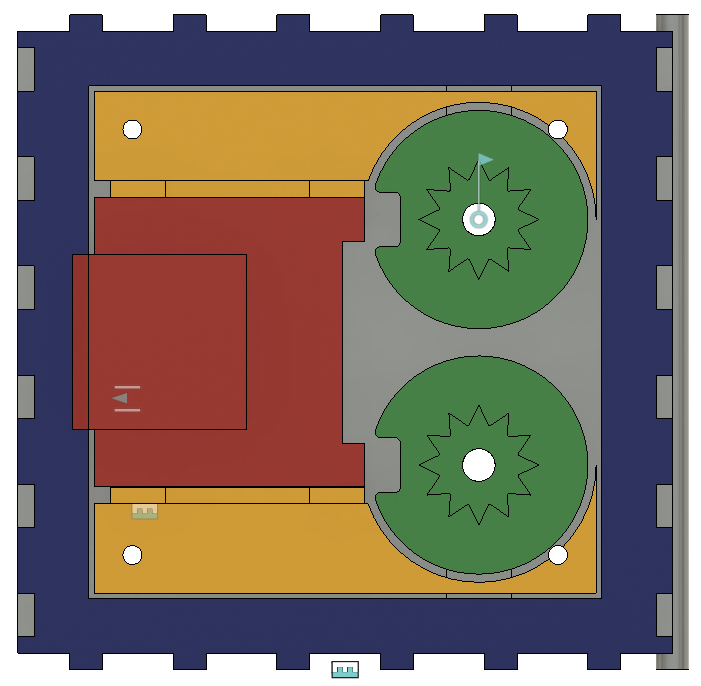
\includegraphics[width=260pt]{kapitoly/obrazky/M1/mechanizmus.png}
    \caption{Zelená barva značí kódová kola, červená západku, modrá pevnou část trezoru a žluté díly tvoří distanci}
    \label{fig:M1-mechanizmus}
\end{figure}
\newpage